\section{Steering Model of the Vehicle}\label{sec:SteeringModel}
After describing a model for the driving part of the vehicle seen on \figref{fig:completeMechanicalDiagram}, the present section draws a model from the steering part, which is isolated in \figref{steeringMechanical}. Thus, the focus is made on the relationship between the PWM command signal to the servo, the angle of the servo, and the resulting orientation of the vehicle. To facilitate the steering modelisation, the vehicle's velocity is considered only around an operating point. A overview of the braking system can be seen in.

 \begin{figure}[H]
 	\centering
 	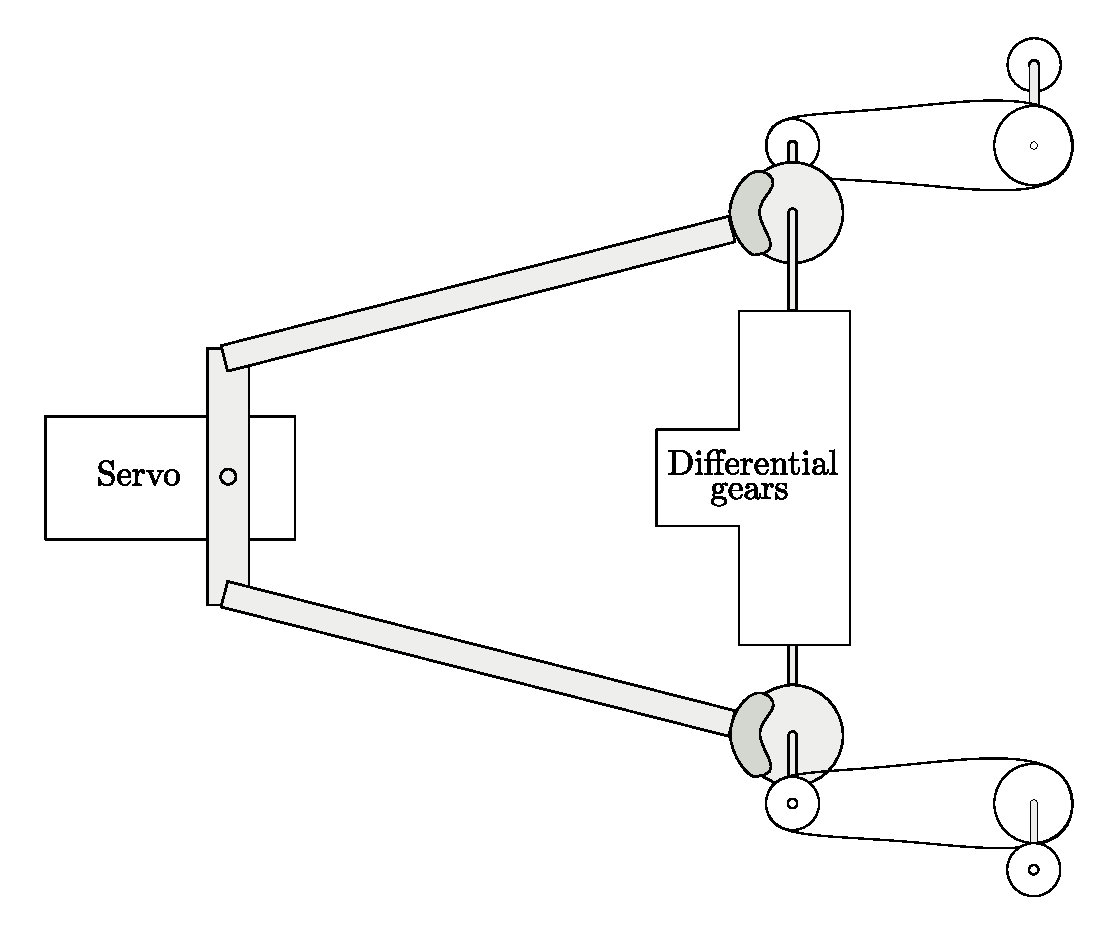
\includegraphics[scale=0.6]{figures/steeringMechanical.pdf}
 	\caption{Mechanical drawing of the steering}
 	\label{steeringMechanical}
 \end{figure}

As described in \secref{sec:Vehicledescription}, when the servo turns one way, it pushes one of the arms, which in turn moves  a brake pad towards the brake disc to add friction and hold the corresponding belt. The differential gears will then transfer the power from one belt to the other.

\subsection{Directional model}
As the steering system contains many moving parts, it is convenient to start with a simple model, to verify it, and iterate until it is satisfactory.\\
%
The first model considered can be seen on \figref{basicSteering}.

\begin{figure}[H]
	\centering
	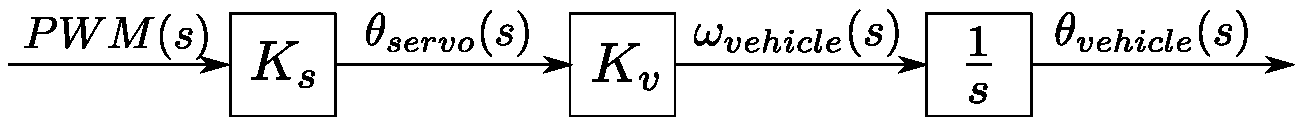
\includegraphics[width=0.8\textwidth]{figures/basicSteeringModel.pdf}
	\caption{A basic steering model}
	\label{basicSteering}
\end{figure}
 
As described in \secref{Servo}, the angle of the servo is proportional to a pulse width modulated signal on its control input (let aside the offset intrinsic to the servomotor). The pulse width is therefore chosen as the input in this model. It is then multiplied by a constant, \si{K_s}, which translates the pulse width to an angle of the servo.
Since the velocity of the vehicle is assumed constant, the rate of change of the direction must be a function of the servo angle, and a constant, \si{K_v}, representing the speed of the vehicle and the braking the system.
The rate of change in the vehicle's angle is finally integrated over time, resulting in a angle heading. 

\subsection{Extension of the Directional Model}

The first model describes in a simple manner how the mechanical part of the steering system functions. However, it can be extended to include the time delay caused by the servo. According to \secref{Servo}, the servo is controlled by a PWM signal with a period of 30 ms. This means, that it will not be possible to update the servo angle continuously, but only in discrete time steps of 30 ms. These steps will be implemented in the model as a sampling delay.\\
As seen in the Modeling and Control course on the 5th semester of Electronic and IT at Aalborg University \cite{KMNielsen}, a delay is usually described in frequency domain by an exponential factor:
\begin{flalign}
  \eq{\mathcal{L}\left[u(t+\lambda)\right]}{U(s)\cdot e^{-\lambda \cdot s}}&&\nonumber
  \label{eq:delaySampling}
\end{flalign}
However, for small values of \si{\lambda}, it is possible to use the approximation:
\begin{flalign}
  \si{e^{-\lambda \cdot s} \sim \frac{1}{\lambda\cdot\text{s}+1}}&&\nonumber
  \label{eq:delaySampling}
\end{flalign}

With the delay from the servo, \si{\lambda}, being \si{30\ ms}, this approximation is used and inserted into the model between the sent PWM and the action of the servo, as shown on \figref{basicSteeringWithDelay}:
\begin{figure}[H]
	\centering
	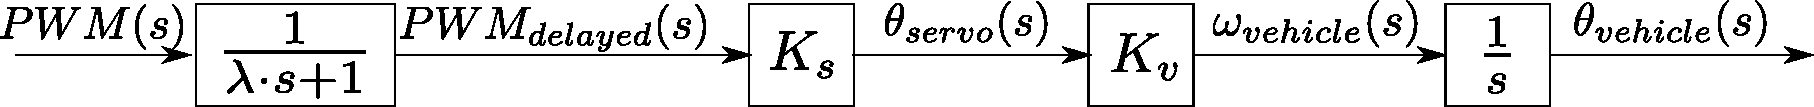
\includegraphics[width=0.8\textwidth]{figures/basicSteeringModelWithDelay.pdf}
	\caption{A basic steering model}
	\label{basicSteeringWithDelay}
\end{figure}
%
This model describes the action of the steering on the vehicle, by translating PWM signals sent to the servo into headings of the vehicle and allows to apply a control on the direction of the vehicle, but not for it to follow a predefined set of points.

\subsection{Line Following Model}
Since the vehicle has to follow a predetermined route, a direction control alone is not enough. As seen on \figref{SteeringDeviation}, any change of direction caused by a disturbance, will cause a deviation from the planned line between two points A and B on the wanted route.

\begin{figure}[H]
	\centering
	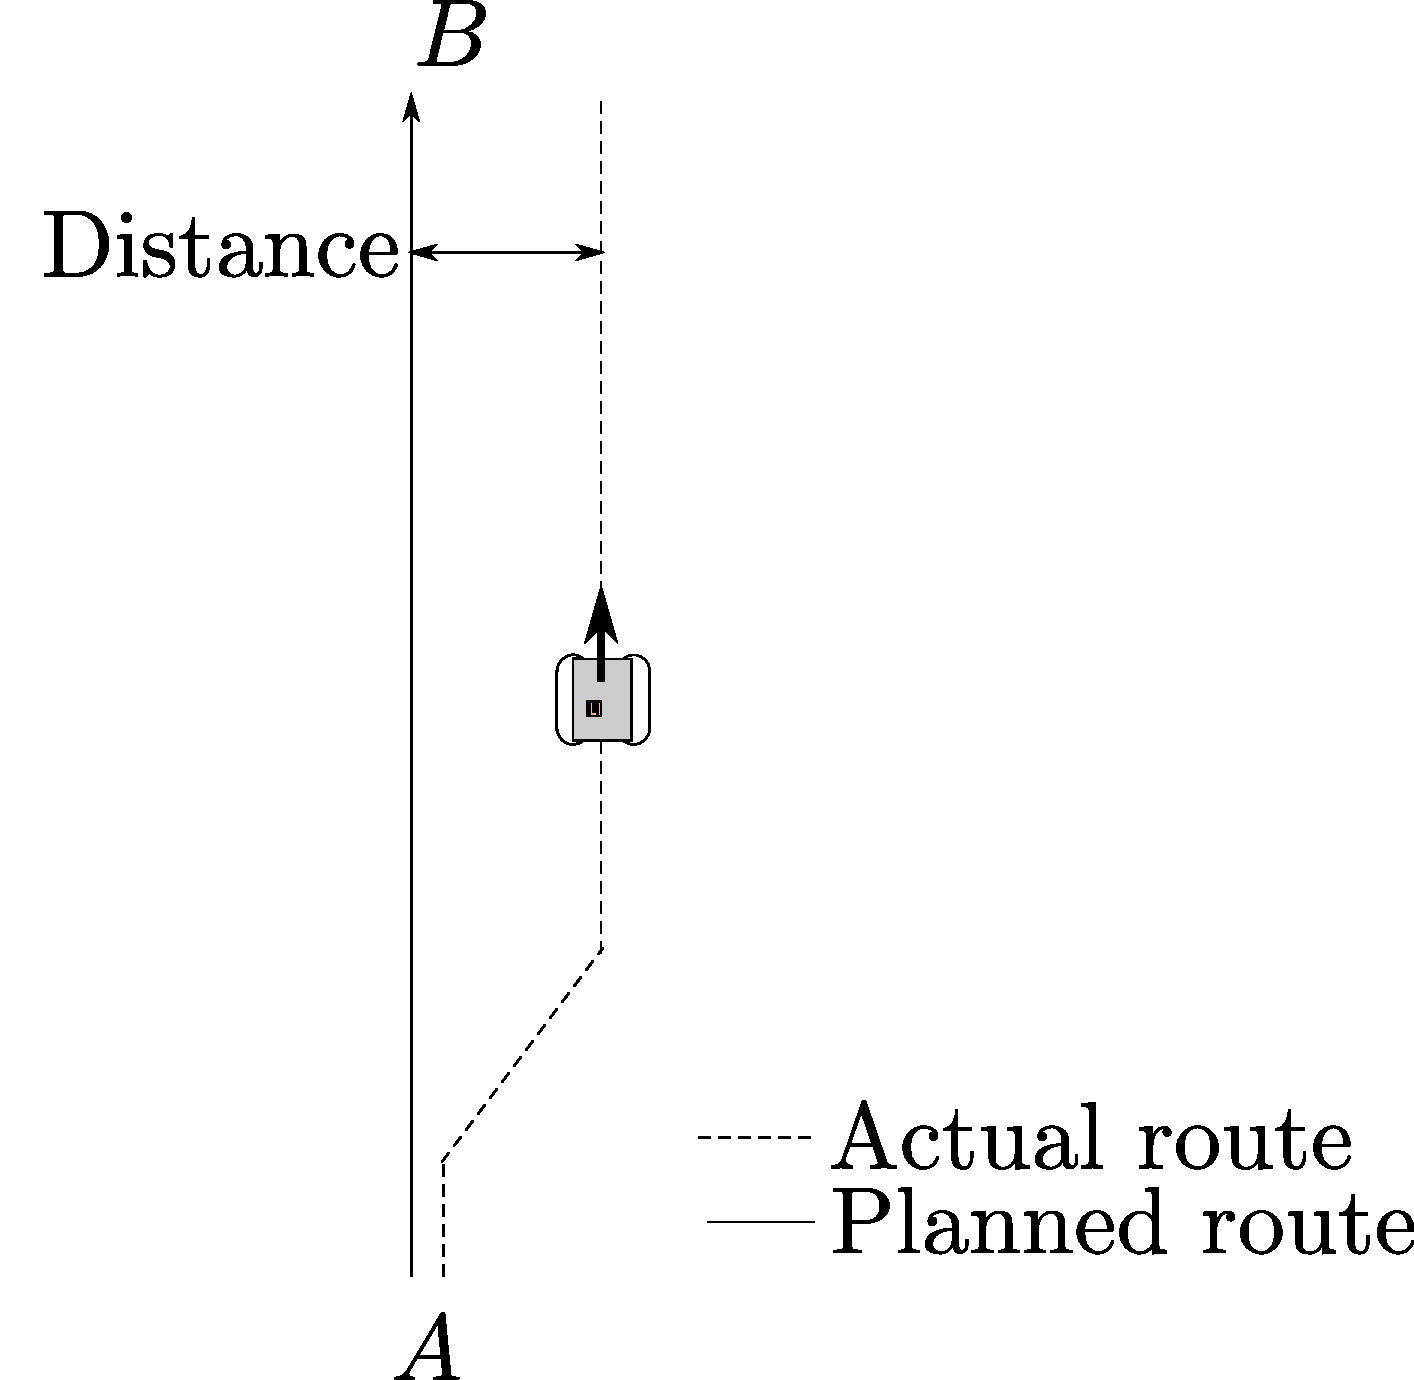
\includegraphics[width=0.6\textwidth]{figures/steeringDeviation.pdf}
	\caption{Consequence of using directional control alone}
	\label{SteeringDeviation}
\end{figure}

How large the deviation is, should depend on the vehicle's erroneous angle from the wanted line, its velocity and the time it takes for the control system to account for the error. Assuming the speed is constant and the measuring and control delays too, the error can then be described as an integration over time of the error angle multiplied with the velocity.